% Please use the skeleton file you have received in the
% invitation-to-submit email, where your data are already
% filled in. Otherwise please make sure you insert your
% data according to the instructions in PoSauthmanual.pdf
\documentclass[a4paper]{PoS}
\usepackage{subfigure}
\newcommand{\GEANTfour} {\textsc{geant4}}

\title{Study of Jet Substructure Variables with the SiFCC Detector at 100 TeV}

\ShortTitle{Study of Jet Substructure Variables with the SiFCC Detector at 100 TeV}

\author{\speaker{C.-H Yeh}$^a$,S.V. Chekanov$^b$ ,A.V. Kotwal$^{c}$,J. Proudfoot$^{b}$,S. Sen$^{c}$,N.V. ~Tran$^{d}$,S.-S Yu$^{a}$\\     
     \llap{$^a$}Department of Physics, National Central University\\
     Chung-Li, Taoyuan City 32001, Taiwan\\
     \llap{$^b$}HEP Division, Argonne National Laboratory\\
     9700 S. Cass Avenue, Argonne, IL 60439, USA\\
     \llap{$^c$}Department of Physics, Duke University\\
     Durham, NC 27708, USA\\
     \llap{$^d$}Fermi National Accelerator Laboratory\\
     Batavia, IL 6051, USA\\
     E-mail:  \email{a9510130375@gmail.com},
     \email{chekanov@anl.gov},
     \email{kotwal@phy.duke.edu},
     \email{sourav.sen@duke.edu},
     \email{ntran@fnal.gov},
     \email{proudfoot@anl.gov},
     \email{syu@phy.ncu.edu.tw}}

\abstract{We study the performance of jet substructure variables with a detector designed for  high energy $pp$ collisions at a 100 TeV collider.  The two-prong jets from Z'$\rightarrow$$WW$ and three-prong jets from Z'$\rightarrow$$t\bar{t}$ are compared with the background from light quark jets, assuming  $Z'$ masses in the range 5 -- 40 TeV.   We present the results on signal efficiency and background rejection using full GEANT simulations.}

\FullConference{The 39th International Conference on High Energy Physics (ICHEP2018)\\
		4-11 July, 2018\\
		Seoul, Korea}


\begin{document}

Particle collisions at energies  beyond those attained at the LHC will lead to many 
challenges for detector technologies.
Future experiments, such as high-energy LHC (HE-LHC),
future circular $pp$ colliders of the European initiative, FCC-hh~\cite{Benedikt:2206376} and the Chinese initiative, SppC~\cite{Tang:2015qga} will be required to measure high-momentum bosons ($W$, $Z$, $H$) and top quarks with strongly
collimated decay products that form jets.  
Therefore, reconstruction of jet substructure  variables for collimated jets with transverse 
momentum above 10 TeV
requires an appropriate calorimeter design.  In particular, the transverse cell size of the hadronic 
calorimeters  (HCALs) is one of the major factors that can significantly impact 
the reconstruction of boosted particles.

To study the transverse segmentuion of HCALs,
\GEANTfour\ (version 10.3) ~\cite{Allison:2016} simulation of calorimeter response are used together
with the full reconstruction of calorimeter clusters formed by the Pandora algorithm~\cite{Marshall:2013,Charles:2009ta}.
The FCC-like detector geometry used in this study is described in~\cite{Chekanov:2016ppq},
while Monte Carlo event simulation samples are available from the
HepSim database ~\cite{Chekanov:2014fga}.

In our study, we simulated the $Z'$ bosons with the center-of-mass energies (c.m.) at 5, 10, 20, and 40 TeV. These particles are forced to decay to two light-flavor jets ($q\bar{q}$) as background, $W W$ or $t\bar{t}$ as signal, where $W$($\rightarrow$$q'\bar{q}$) and $t$($ \rightarrow  W^+\>b \rightarrow q'\bar{q} b$) decay hadronically. We use different configurations of calorimeter geometry to see whether the smallest configuration can give the best separation power to distinguish signal from background in different jet substructures. We draw the receiver operating characteristic (ROC) curves to quantify the detector performance and find out the cell size that can give the best separation power.

We use soft drop declustering~\cite{Larkoski:2014wba} to study the performance of detector with various detector cell sizes and c.m. energies. Figure~\ref{1}(a) shows the representative ROC curves for the soft-drop mass~\cite{Larkoski:2014wba} for three detector cell sizes at 20 TeV with $\beta=0$. For $\beta=0$, the smallest detector cell size, $1~\mathrm{cm}\times1~\mathrm{cm}$, has the best separation power at $\sqrt{s}=$5, 10, and 20 TeV when the signal is $Z' \rightarrow WW$ and at $\sqrt{s}=$10 and 20 TeV when the signal is $Z' \rightarrow$ $t\bar{t}$. For $\beta=2$, the smallest detector cell size does not have improvements in the separation power with respect to those with larger cell sizes.

We also use several jet substructure variables, including $N$-subjettiness~\cite{Thaler:2010tr} and energy correlation function~\cite{Larkoski:2013eya} to study. The signals considered are $Z'\rightarrow WW$ ($\tau_{21}$,$C_2^1$) and $Z' \rightarrow t\bar{t}$ ($\tau_{32}$). Figure~\ref{1}(b) shows the ROC curves for the tau21~\cite{Thaler:2010tr} using three HCAL sizes for jets at 20 TeV. For all of them, the smallest detector cell size ($1\times1~\mathrm{cm}^2$) does not have the best separation power. It is interesting to note that at very large c.m. energies, the large detector cell sizes have a better separation power than the smallest cell size in most of cases. 

In conclusion, HCALs that use the cell sizes of $20\times 20$~cm$^2$ ($\Delta \eta \times \Delta \phi = 0.1\times0.1$) 
are least performant almost for several studied 
substructure variables for jet transverse momenta between 2.5 to 10~TeV. 
Such cell sizes are close to 
those used for the ATLAS and CMS detectors at the LHC. 
In terms of the reconstruction of the physics-motivated quantities  
used for jet substructure studies, the  performance 
of a  hadronic callorimeter  with 
$\Delta \eta \times \Delta \phi = 0.022\times0.022$ is, in most cases,
better than for a detector with  $0.1\times0.1$ cells.
Thus this study confirms the  baseline SiFCC detector geometry \cite{Chekanov:2016ppq}
that uses $\Delta \eta \times \Delta \phi = 0.022\times0.022$ HCAL cells.


\begin{figure}
\begin{center}
 \subfigure[Soft drop mass with $\beta=0$ and 20 TeV] {
 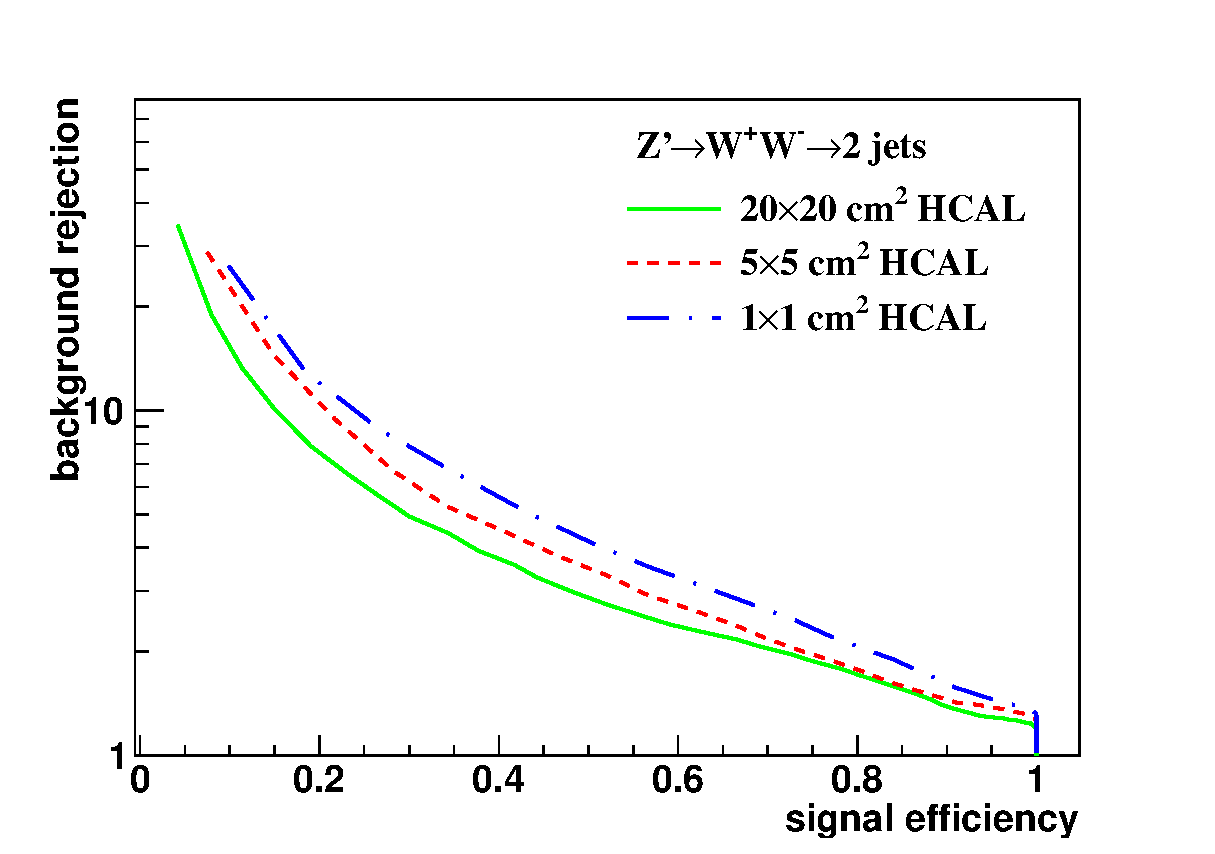
\includegraphics[width=0.4\textwidth]{A_Cluster_mass_mmdt_20tev_eff_1_central_fix_at_Median_bin_ww_qq_log_no_UOF.eps}
 }
 \subfigure[$\tau_{21}$ with 20 TeV] {
 \includegraphics[width=0.4\textwidth]{Rawhit_05GeV_tau21_20tev_eff_1_New2_after_cut_25bins_no_UOF_new_75pa.eps}
 }
\end{center}
\caption{The representative pictures of ROC curves with different jet substructure variables and energies.}
\label{1}
\end{figure}

\begin{thebibliography}{99}
%%%
\bibitem{Benedikt:2206376} 
  A.~J.~Larkoski, S.~Marzani, G.~Soyez and J.~Thaler,
  \emph{The Global Future Circular Colliders Effort},
  CERN-ACC-SLIDES-2016-0016
  [JCERN-ACC-SLIDES-2016-0016. Presented at P5 Workshop on the Future of High Energy Physics, BNL, USA, Dec. 15-18,  2013].
%%%
\bibitem{Tang:2015qga} 
  J.~Tang {\it et al.},
  \emph{Concept for a Future Super Proton-Proton Collider},
  arXiv:1507.03224 [physics.acc-ph]
%%%
\bibitem{Allison:2016} 
  J.~Allison {\it et al.},
  \emph{Recent developments in Geant4},
  \emph{Nucl.\ Instrum.\ Meth.\ A} {\bf 835}, 186 (2016).
  doi:10.1016/j.nima.2016.06.125
%%%
\bibitem{Marshall:2013} 
  J.~S.~Marshall and M.~A.~Thomson,
  \emph{Pandora Particle Flow Algorithm},
  arXiv:1308.4537 [physics.ins-det].
%%%
%\cite{Charles:2009ta}
\bibitem{Charles:2009ta} 
  M.~J.~Charles,
   \emph{PFA Performance for SiD,}
  arXiv:0901.4670 [physics.data-an].
\bibitem{Chekanov:2016ppq} 
  S.~V.~Chekanov, M.~Beydler, A.~V.~Kotwal, L.~Gray, S.~Sen, N.~V.~Tran, S.-S.~Yu and J.~Zuzelski,
  \emph{Initial performance studies of a general-purpose detector for multi-TeV physics at a 100 TeV pp collider},
  \emph{JINST} {\bf 12}, no. 06, P06009 (2017)
  doi:10.1088/1748-0221/12/06/P06009
  [arXiv:1612.07291 [hep-ex]].
%%%
\bibitem{Chekanov:2014fga} 
  S.~V.~Chekanov,
  \emph{HepSim: a repository with predictions for high-energy physics experiments},
  \emph{Adv. High Energy Phys.}  {\bf 2015}, 136093 (2015)
  doi:10.1155/2015/136093
  [arXiv:1403.1886 [hep-ph]].
%%%
\bibitem{Larkoski:2014wba} 
  A.~J.~Larkoski, S.~Marzani, G.~Soyez and J.~Thaler,
  \emph{Soft Drop},
  \emph{JHEP} {\bf 1405}, 146 (2014)
  doi:10.1007/JHEP05(2014)146
  [arXiv:1402.2657 [hep-ph]].
%%%
\bibitem{Thaler:2010tr} 
  J.~Thaler and K.~Van Tilburg,
  \emph{Identifying Boosted Objects with N-subjettiness},
  \emph{JHEP} {\bf 1103}, 015 (2011)
  doi:10.1007/JHEP03(2011)015
  [arXiv:1011.2268 [hep-ph]].
%%%
\bibitem{Larkoski:2013eya} 
  A.~J.~Larkoski, G.~P.~Salam and J.~Thaler,
  `\emph{Energy Correlation Functions for Jet Substructure},
  \emph{JHEP} {\bf 1306}, 108 (2013)
  doi:10.1007/JHEP06(2013)108
  [arXiv:1305.0007 [hep-ph]].
%%%
\end{thebibliography}

\end{document}
